\documentclass[a4paper]{article}
\usepackage{float}
\usepackage[spanish,es-tabla]{babel}
\usepackage[T1]{fontenc}
\usepackage[spanish]{babel}
\usepackage{graphicx} 
\usepackage[utf8]{inputenc}
\usepackage{amsmath}
\usepackage{longtable}
\usepackage{graphicx}
\usepackage[colorinlistoftodos]{todonotes}
\usepackage[letterpaper,top=2.5cm,bottom=2.5cm,left=2cm,right=2cm,marginparwidth=2.5cm]{geometry}
\renewcommand{\baselinestretch}{1.25}


\title{Informe Física 2}
\author{Danny Córdova, Edwin Dávila}
\date{21 de Febrero de 2023}



\begin{document}

\maketitle

\section{Introducción}
En la presente práctica se hizo un estudio sobre la cinemática. Se estudió como se comporta un cuerpo bajo movimiento rectilíneo uniforme en un experimento controlado. Se realizaron 48 mediciones para poder realizar un gráfico de velocidad final sobre tiempo y otro de distancia sobre tiempo. El objetivo principal de esta práctica es encontrar una regresión lineal de la velocidad y una regresión cuadrática de la distancia para que se comprueben las fórmulas de la cinemática. 

\section{Metodología experimental}
Para este experimento se usó un riel de metal para colocar un móvil, el móvil, una aspiradora invertida para quitar la mayor cantidad de fricción posible y un instrumento digital para medir el tiempo, velocidades instantáneas y aceleración promedio. El instrumento digital contaba con 2 sensores, uno se colocó en una distancia fija en el riel correspondiente a 20cm y el otro se colocó en un inicio en 120 cm y luego se fue restando 2 cm por cada medición hasta llegar a los 24 cm (en total se realizaron 48 mediciones). 

Las unidades usadas en este informe son las del SI (Sistema Internacional). Las unidades fundamentales usadas son el metro (m) y sus subunidades para longitudes y los segundos (s) y sus subunidades para el tiempo. Las unidades derivadas son las velocidad, medida en $cm/s$; y la aceleración, medida en $cm/s^2$.
Las variables directas de este experimento son: 
\begin{enumerate}
    \item El tiempo
    \item La distancia
\end{enumerate}   
Sin embargo, el dispositivo usado para medir el tiempo hacía el trabajo de medir las variables indirectas de: 
\begin{enumerate}
    \item Velocidad inicial
    \item Velocidad final
    \item Aceleración
\end{enumerate}
En la práctica se realizaron 50 mediciones, cada una con 

Las fórmulas usadas en esta práctica son: 

\begin{equation}
    y=mx+b
\end{equation}
esta fórmula representa la ecuación de una recta y sirve para hacer la regresión lineal. Aquí x es la variable independiente y y la variable dependiente. 

\begin{equation}
   m=\frac{\sum x_i*y_i-\frac{1}{n}\sum x_i \sum y_i}{\sum x_i^2-\frac{1}{n}(\sum x_i)^2} 
\end{equation}
donde m es la pendiente de la regresión lineal y n es el número de datos.

\begin{equation}
    b=\frac{\sum y_i}{n}-m\frac{\sum x_i}{n}
\end{equation}
donde b es el corte en el eje y de la regresión lineal.

\begin{equation}
    y=c_0+c_1x+c_2x^2
\end{equation}
esta fórmula representa la ecuación cuadrática y sirve para la regresión polinómica de grado 2, dónde $c_0$, $c_1$ y $c_2$ son coeficientes a encontrar.

    \[a_0(n)+a_1\sum x_i+a_2\sum (x_i)^2=\sum y_i\]
    \[a_0\sum x_i+a_1\sum (x_i)^2+a_2\sum (x_i)^3=\sum x_i\sum y_i\]
    \begin{equation}
        a_0\sum (x_i)^2+a_1\sum (x_i)^3+a_2\sum (x_i)^4=\sum (x_i)^2\sum y_i
    \end{equation}\
con ayuda de esta fórmula se pueden deducir los resultados de los coeficientes $c_0$, $c_1$ y $c_2$ para hallar la fórmula de la regresión polinómica de grado 2.

\begin{equation}
    \epsilon=\frac{|x_{exp}-x_{teo}|}{x_{teo}}\times100\%
\end{equation}
  donde $\epsilon$ es el error porcentual, $x_{exp}$ el valor de dato experimental y $x_{teo}$ el valor del dato teórico.

\section{Resultados y observaciones}
A partir de la Tabla 1 adjuntada en anexos, se tienen los siguientes gráficos:
\begin{figure} [H]
    \centering
    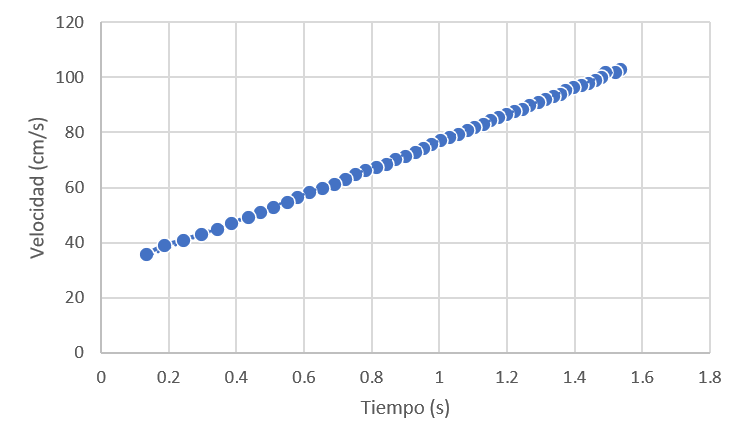
\includegraphics{Figura_Vf_sobre_t(1).png}
    \caption{Velocidad final sobre tiempo}
    \label{fig:v_t}
\end{figure}
\begin{figure} [H]
    \centering
    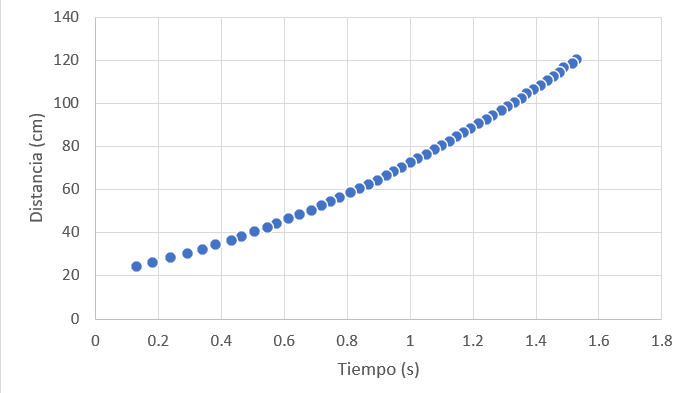
\includegraphics{Figura_x_sobre_t(1).png}
    \caption{Distancia sobre tiempo}
    \label{fig:x_t}
\end{figure}

A partir de las ecuaciones (1), (2) y (3), calculamos la ecuación que representa la regresión lineal de los datos de Figura 1 (velocidad final sobre tiempo) y obtenemos:
\[V_f(t) = 48.351(t) + 28.603\]
Por lo que la $a=48.351 cm/s^2$ y la $V_o=28.603m/s$.

Ahora, a partir de las ecuaciones (4) y (5) hallamos la regresión polinómica de grado 2 que representa los datos de la Figura 2 y obtenemos:
\[x(t)=25.2t^2 + 26.433t + 20.03\]
Por lo que $a=50.4 cm/s^2$, la $V_o=26.433 m/s$ y la $x_o=20,03 cm$

Usando la fórmula (6), calculamos el error porcentual y obtenemos:
\[\epsilon_{x_o}=\frac{|x_{exp}-x_{teo}|}{x_{teo}}\]
\[\epsilon_{x_o}=1.50\%\]
\[\epsilon_{V_o}=11.1\%\]
\[\epsilon_{a}=3.85\%\]
\section{Conclusiones}
Podemos notar que el promedio de los valores experimentales obtenidos en el laboratorio y los teóricos obtenidos mediante el uso de regresión lineal tienen un error porcentual muy bajo, por lo que podemos asegurarnos que las leyes de la cinemática en el movimiento rectilíneo uniforme son válidas. Los errores se deben principalmente a la relativamente poca cantidad de mediciones que se realizaron, a los errores en la colocación de los sensores y a la incertidumbre propia de los instrumentos de medición. De manera general, los objetivos de esta práctica se cumplieron satisfactoriamente y los cálculos salieron como se esperaban.


\section{Referencias}
Herrera, N. (2018). \textit{Cinemática de traslación.}
\section{Anexos}

\begin{longtable}{|c|c|c|c|c|c|c|}   
\caption{Datos medidos en el experimento} \label{tab:longdatos} \\

    \hline  \multicolumn{1}{|c|}{x} &  \multicolumn{1}{|c|}{$t_1$ (ms)} &  \multicolumn{1}{|c|}{t (s)} &  \multicolumn{1}{|c|}{$t_2$ (ms)} &  \multicolumn{1}{|c|}{$V_o$($\frac{cm}{s})$} &  \multicolumn{1}{|c|}{$V_f$($\frac{cm}{s}$)} &  \multicolumn{1}{|c|}{a($\frac{cm}{s^2}$) } 
    \endfirsthead

    \multicolumn{7}{c}%
    {{\bfseries \tablename\ \thetable{} -- continuación de la página anterior}} \\
     \hline  \multicolumn{1}{|c|}{x} &  \multicolumn{1}{|c|}{$t_1$ (ms)} &  \multicolumn{1}{|c|}{t (s)} &  \multicolumn{1}{|c|}{$t_2$ (ms)} &  \multicolumn{1}{|c|}{$V_o$($\frac{cm}{s})$} &  \multicolumn{1}{|c|}{$V_f$($\frac{cm}{s}$)} &  \multicolumn{1}{|c|}{a($\frac{cm}{s^2}$) } 
    \endhead

\hline \multicolumn{7}{|r|}{{Continúa en la siguiente página}} \\ \hline
\endfoot

\hline \hline
\endlastfoot
    \hline
        120 & 99,45 & 1,533 & 29,07 & 30,2 & 103 & 47,7 \\ \hline
        118 & 100,0 & 1,519 & 29,43 & 30,0 & 102 & 47,3 \\ \hline
        116 & 99,31 & 1,491 & 29,53 & 30,2 & 102 & 47,9 \\ \hline
        114 & 99,78 & 1,477 & 29,98 & 30,1 & 100 & 47,4 \\ \hline
        112 & 99,85 & 1,460 & 30,31 & 30,0 & 99 & 47,2 \\ \hline
        110 & 100,1 & 1,440 & 30,58 & 30,0 & 98,1 & 47,3 \\ \hline
        108 & 100,2 & 1,418 & 30,87 & 29,9 & 97,2 & 47,4 \\ \hline
        106 & 99,62 & 1,394 & 31,09 & 30,1 & 96,5 & 47,6 \\ \hline
        104 & 99,59 & 1,372 & 31,43 & 30,1 & 95,5 & 47,6 \\ \hline
        102 & 100,2 & 1,356 & 31,87 & 29,9 & 94,1 & 47,3 \\ \hline
        100 & 99,84 & 1,335 & 32,22 & 30,0 & 93,1 & 47,2 \\ \hline
        98,0 & 99,74 & 1,312 & 32,6 & 30,1 & 92 & 47,2 \\ \hline
        96,0 & 100,4 & 1,293 & 33 & 29,9 & 90,9 & 47,2 \\ \hline
        94,0 & 99,69 & 1,266 & 33,41 & 30,1 & 89,8 & 47,1 \\ \hline
        92,0 & 99,83 & 1,245 & 33,82 & 30,1 & 88,7 & 47,1 \\ \hline
        90,0 & 99,81 & 1,220 & 34,21 & 30,1 & 87,7 & 47,2 \\ \hline
        88,0 & 99,73 & 1,196 & 34,63 & 30,1 & 86,6 & 47,3 \\ \hline
        86,0 & 99,82 & 1,174 & 35,11 & 30,1 & 85,5 & 47,2 \\ \hline
        84,0 & 99,65 & 1,150 & 35,56 & 30,1 & 84,4 & 47,2 \\ \hline
        82,0 & 99,89 & 1,128 & 36,08 & 30,0 & 83,2 & 47,1 \\ \hline
        80,0 & 99,97 & 1,103 & 36,6  & 30,0 & 82 & 47,1 \\ \hline
        78,0 & 100,1 & 1,081 & 37,08 & 30,0 & 80,9 & 47,2 \\ \hline
        76,0 & 100,1 & 1,054 & 37,69 & 30,0 & 79,6 & 47,1 \\ \hline
        74,0 & 100,1 & 1,028 & 38,31 & 30,0 & 78,3 & 47,0 \\ \hline
        72,0 & 100,2 & 1,003 & 38,91 & 30,0 & 77,1 & 47,0 \\ \hline
        70,0 & 99,90 & 0,9751 & 39,54 & 30,0 & 75,9 & 47,0 \\ \hline
        68,0 & 99,62 & 0,9511 & 40,30 & 30,1 & 74,4 & 46,6 \\ \hline
        66,0 & 100,3 & 0,9270 & 41,18 & 29,9 & 72,8 & 46,3 \\ \hline
        64,0 & 99,98 & 0,8987 & 41,87 & 30,0 & 71,6 & 46,3 \\ \hline
        62,0 & 100,2 & 0,8693 & 42,72 & 29,9 & 70,2 & 46,3 \\ \hline
        60,0 & 100,4 & 0,8427 & 43,68 & 29,9 & 68,7 & 46,1 \\ \hline
        58,0 & 100,4 & 0,8139 & 44,56 & 29,9 & 67,3 & 46,0 \\ \hline
        56,0 & 100,3 & 0,7800 & 45,24 & 29,9 & 66,3 & 46,7 \\ \hline
        54,0 & 100,9 & 0,7514 & 46,28 & 29,7 & 64,8 & 46,7 \\ \hline
        52,0 & 101,0 & 0,7199 & 47,60 & 29,7 & 63,0 & 46,3 \\ \hline
        50,0 & 101,3 & 0,6886 & 48,86 & 29,6 & 61,4 & 46,2 \\ \hline
        48,0 & 100,9 & 0,6522 & 50,16 & 29,7 & 59,8 & 46,1 \\ \hline
        46,0 & 100,2 & 0,6158 & 51,46 & 30,0 & 58,3 & 46,0 \\ \hline
        44,0 & 100,1 & 0,5793 & 53,02 & 30,0 & 56,6 & 46,0 \\ \hline
        42,0 & 100,9 & 0,5488 & 54,73 & 29,7 & 54,8 & 45,7 \\ \hline
        40,0 & 101,0 & 0,5085 & 56,79 & 29,7 & 52,8 & 45,5 \\ \hline
        38,0 & 100,7 & 0,4687 & 58,74 & 29,8 & 51,1 & 45,4 \\ \hline
        36,0 & 101,0 & 0,4349 & 60,77 & 29,7 & 49,4 & 45,2 \\ \hline
        34,0 & 101,1 & 0,3852 & 63,74 & 29,7 & 47,1 & 45,2 \\ \hline
        32,0 & 101,3 & 0,3429 & 66,60 & 29,6 & 45,0 & 45,0 \\ \hline
        30,0 & 101,0 & 0,2945 & 69,81 & 29,7 & 43,0 & 45,1 \\ \hline
        28,0 & 100,1 & 0,2427 & 73,44 & 30,0 & 40,8 & 44 \\ \hline
        26,0 & 98,21 & 0,1859 & 76,56 & 30,5 & 39,2 & 46,5 \\ \hline
        24,0 & 100,1 & 0,1331 & 83,27 & 30,0 & 36,0 & 45,5  \\ \hline
   
\end{longtable}


\end{document}
